% ============================================================================
%  অধ্যায় ৭ : ত্রিকোণমিতি ১
%  COMPILE WITH XeLaTeX  (twice, so the point total resolves)
%  Overleaf: Menu -> Compiler -> XeLaTeX
%  Requires: bnhandout.sty  and  fonts/Kalpurush.ttf  in the project
% ============================================================================
\documentclass[11pt]{article}
\usepackage{bnhandout}

\usepackage{amsmath}
\usepackage{amssymb}
\usepackage{tikz}

\hauthor[https://jugantordey.github.io/]{Jugantor Dey}
\hseries{\textit{Mathematics for the Physics Olympiad}}

\begin{document}

\handouttitle{Chapter 7 : Trigonometry I }

\noindent
এই অধ্যায়ে ঢোকার আগে অধ্যায় ৫ (Euclidean Geometry I) ও অধ্যায় ৬
(Coordinate Geometry I) শেষ করে নাও। ৫ থেকে লাগবে সদৃশ ত্রিভুজ, পিথাগোরাস আর
সমবাহু ত্রিভুজের ধর্ম; ৬ থেকে লাগবে কার্তেসীয় সমতল, দূরত্ব সূত্র আর বৃত্তের
সমীকরণ। অধ্যায় ৪-এর domain ও range-এর ভাষাটাও এক জায়গায় কাজে লাগবে।

স্কুলে ত্রিকোণমিতি শেখানো হয় একগাদা সূত্র মুখস্থ করার বিষয় হিসেবে। এই
অধ্যায়ের উদ্দেশ্য ঠিক উল্টো। এখানে মোটে দুটি জিনিস মনে রাখতে হবে: একক
বৃত্তের ছবিটি, আর যোগ সূত্র দুটি। বাকি প্রতিটি সূত্র ওই দুটি থেকে দুই-তিন
লাইনে বেরিয়ে আসে, আর সেটাই নিচে করে দেখানো হয়েছে। কোনো সূত্র ভুলে গেলে
আতঙ্কিত হওয়ার কিছু নেই; আবার বের করে নাও।

তিনটি ধারণা এই অধ্যায়ের মেরুদণ্ড। প্রথমত, $\sin$ ও $\cos$ ত্রিভুজের ধর্ম
নয়, কোণের ফাংশন; ত্রিভুজ কেবল প্রথম দিকে হিসাব করার একটি মই, যা পরে ফেলে দেওয়া
হবে। দ্বিতীয়ত, একক বৃত্ত এই ফাংশনগুলোকে সমকোণের বাইরে, এমনকি ঋণাত্মক কোণেও
বাড়িয়ে দেয়। তৃতীয়ত, radian কোনো খেয়ালি একক নয়; ওটাই স্বাভাবিক একক, আর কেন
স্বাভাবিক সেটাও দেখানো হবে।

এই অধ্যায়ে মোট \totalpoints\ পয়েন্ট আছে।

% ============================================================================
\section{ত্রিভুজ থেকে অনুপাত}
% ============================================================================

\begin{idea}[সমকোণী ত্রিভুজে ছয়টি অনুপাত]
একটি সমকোণী ত্রিভুজের একটি সূক্ষ্মকোণ $\theta$ ধরো। সমকোণের বিপরীত বাহুটির নাম
অতিভুজ (hypotenuse); $\theta$-এর বিপরীত বাহুটির নাম লম্ব (opposite); আর
$\theta$-সংলগ্ন বাকি বাহুটির নাম ভূমি (adjacent)। তাহলে
\[
  \sin\theta = \frac{\text{লম্ব}}{\text{অতিভুজ}}, \qquad
  \cos\theta = \frac{\text{ভূমি}}{\text{অতিভুজ}}, \qquad
  \tan\theta = \frac{\text{লম্ব}}{\text{ভূমি}} .
\]
এদের বিপ্রতীপ তিনটির আলাদা নাম আছে:
\[
  \csc\theta = \frac{1}{\sin\theta}, \qquad
  \sec\theta = \frac{1}{\cos\theta}, \qquad
  \cot\theta = \frac{1}{\tan\theta} .
\]
সংজ্ঞা থেকেই সরাসরি পাওয়া যায় $\tan\theta = \dfrac{\sin\theta}{\cos\theta}$,
কারণ লব ও হরে অতিভুজ কেটে যায়।
\end{idea}

\begin{center}
\begin{tikzpicture}[scale=1.0]
  \draw[line width=1pt] (0,0) -- (4,0) -- (4,2.6) -- cycle;
  \draw (3.65,0) rectangle (4,0.35);
  \node[below] at (2,0) {ভূমি};
  \node[right] at (4,1.3) {লম্ব};
  \node[above left] at (2,1.3) {অতিভুজ};
  \draw (0.8,0) arc (0:33:0.8);
  \node at (1.05,0.25) {$\theta$};
\end{tikzpicture}
\end{center}

\begin{idea}[অনুপাতগুলো ত্রিভুজের উপর নির্ভর করে না]
একই কোণ $\theta$ নিয়ে যতগুলো খুশি ভিন্ন মাপের সমকোণী ত্রিভুজ আঁকো; উপরের ছয়টি
অনুপাতের মান সব ত্রিভুজেই এক হবে। তাই ``$\theta$ কোণের sine'' কথাটা অর্থপূর্ণ,
আর $\sin$ সত্যিই কোণের একটি function।
\end{idea}

\noindent
\textbf{প্রমাণ।} $\theta$ সূক্ষ্মকোণবিশিষ্ট দুটি সমকোণী ত্রিভুজ নাও। দুটিতেই
একটি কোণ সমকোণ, আর একটি কোণ $\theta$। দুটি কোণ সমান হলেই ত্রিভুজ দুটি সদৃশ
(অধ্যায় ৫), কারণ তৃতীয় কোণটিও তখন আপনা থেকেই সমান হয়ে যায়:
$180^\circ - 90^\circ - \theta$।

সদৃশ ত্রিভুজে অনুরূপ বাহুর অনুপাত সমান। তাই এক ত্রিভুজে লম্ব ও অতিভুজের অনুপাত
আর অন্য ত্রিভুজে লম্ব ও অতিভুজের অনুপাত সমান, অর্থাৎ $\sin\theta$ দুই ত্রিভুজে
এক। বাকি পাঁচটির যুক্তিও অবিকল একই। $\blacksquare$

\begin{remark}
এই ছোট প্রমাণটিই আসলে গোটা ত্রিকোণমিতির ভিত। এটি না থাকলে ``$\sin 30^\circ$-এর
মান কত'' প্রশ্নটার কোনো উত্তরই হতো না, কারণ প্রতিটি ত্রিভুজ ভিন্ন উত্তর দিত।

স্কুলে যে ``ট্যাড়া লম্বা ভূত'' জাতীয় ছড়া মুখস্থ করানো হয়, সেটা কেবল কোন বাহু কোথায় বসবে
তা মনে রাখার কৌশল; সেটা সংজ্ঞা নয়, আর গণিতও নয়। গণিতটা উপরের সদৃশতার যুক্তিটুকু।
\end{remark}

\begin{example}
একটি সমকোণী ত্রিভুজের বাহু তিনটি $3$, $4$ ও $5$ একক, আর $\theta$ হলো $3$ একক
বাহুটির বিপরীত কোণ। ছয়টি অনুপাতই বের করো।
\end{example}

\begin{solbox}
অতিভুজ সবচেয়ে বড় বাহু, অর্থাৎ $5$। $\theta$-এর বিপরীত বাহু $3$, তাই লম্ব $= 3$
আর ভূমি $= 4$। সুতরাং
\[
  \sin\theta = \tfrac{3}{5}, \qquad
  \cos\theta = \tfrac{4}{5}, \qquad
  \tan\theta = \tfrac{3}{4},
\]
\[
  \csc\theta = \tfrac{5}{3}, \qquad
  \sec\theta = \tfrac{5}{4}, \qquad
  \cot\theta = \tfrac{4}{3} .
\]
লক্ষ করো $\sin\theta$ ও $\cos\theta$ দুটিই $1$-এর চেয়ে ছোট। এটা কাকতালীয় নয়:
অতিভুজ সবসময়ই বাকি দুই বাহুর চেয়ে বড়, তাই ওই দুটি অনুপাত কখনো $1$ ছাড়াতে
পারে না।
\end{solbox}

\begin{idea}[বিশেষ কোণের সঠিক মান]
দুটি বিশেষ ত্রিভুজ থেকে $30^\circ$, $45^\circ$ ও $60^\circ$-এর মান হাতে তুলে
নেওয়া যায়, কোনো calculator ছাড়াই।

\emph{সমদ্বিবাহু সমকোণী ত্রিভুজ :} দুই বাহু $1$ ও $1$ নিলে দুটি সূক্ষ্মকোণই
$45^\circ$, আর পিথাগোরাসে অতিভুজ $\sqrt{2}$।

\emph{অর্ধেক সমবাহু ত্রিভুজ :} $2$ বাহুবিশিষ্ট একটি সমবাহু ত্রিভুজের এক শীর্ষ
থেকে বিপরীত বাহুর উপর লম্ব টানো। লম্বটি ওই বাহুকে সমদ্বিখণ্ডিত করে
(অধ্যায় ৫), তাই একটি অর্ধাংশ পাই যার ভূমি $1$, অতিভুজ $2$, আর কোণ দুটি
$30^\circ$ ও $60^\circ$। পিথাগোরাস অনুযায়ী উচ্চতা $\sqrt{4-1} = \sqrt{3}$।
\end{idea}

\begin{center}
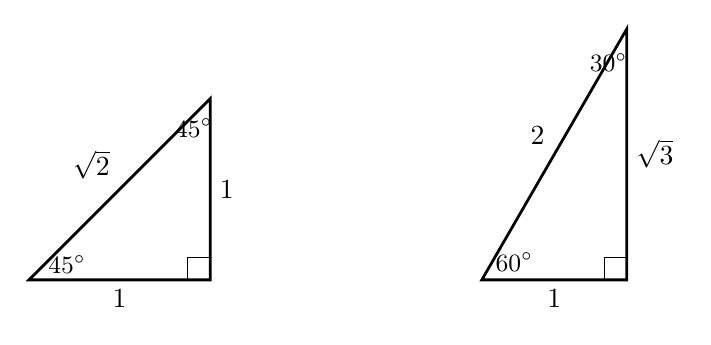
\begin{tikzpicture}[scale=1.15]
  \draw[line width=1pt] (0,0) -- (2,0) -- (2,2) -- cycle;
  \draw (1.75,0) rectangle (2,0.25);
  \node[below] at (1,0) {$1$};
  \node[right] at (2,1) {$1$};
  \node[above left] at (1,1) {$\sqrt{2}$};
  \node at (0.42,0.17) {\small $45^\circ$};
  \node at (1.82,1.68) {\small $45^\circ$};
  \begin{scope}[xshift=5cm]
    \draw[line width=1pt] (0,0) -- (1.6,0) -- (1.6,2.77) -- cycle;
    \draw (1.35,0) rectangle (1.6,0.25);
    \node[below] at (0.8,0) {$1$};
    \node[right] at (1.6,1.39) {$\sqrt{3}$};
    \node[above left] at (0.8,1.39) {$2$};
    \node at (0.36,0.2) {\small $60^\circ$};
    \node at (1.4,2.4) {\small $30^\circ$};
  \end{scope}
\end{tikzpicture}
\end{center}

\begin{example}
উপরের দুটি ত্রিভুজ থেকে $\sin$, $\cos$ ও $\tan$-এর মান পড়ে নাও।
\end{example}

\begin{solbox}
প্রথম ত্রিভুজ থেকে, $45^\circ$-এর লম্ব $1$ ও ভূমি $1$, অতিভুজ $\sqrt{2}$:
\[
  \sin 45^\circ = \frac{1}{\sqrt{2}}, \qquad
  \cos 45^\circ = \frac{1}{\sqrt{2}}, \qquad
  \tan 45^\circ = 1 .
\]

দ্বিতীয় ত্রিভুজে $30^\circ$ কোণটির বিপরীত বাহু $1$, সংলগ্ন বাহু $\sqrt{3}$,
অতিভুজ $2$:
\[
  \sin 30^\circ = \frac{1}{2}, \qquad
  \cos 30^\circ = \frac{\sqrt{3}}{2}, \qquad
  \tan 30^\circ = \frac{1}{\sqrt{3}} .
\]

একই ত্রিভুজে $60^\circ$ কোণটির বেলায় লম্ব ও ভূমি জায়গা বদল করে:
\[
  \sin 60^\circ = \frac{\sqrt{3}}{2}, \qquad
  \cos 60^\circ = \frac{1}{2}, \qquad
  \tan 60^\circ = \sqrt{3} .
\]

লক্ষ করো $\sin 30^\circ = \cos 60^\circ$ এবং $\sin 60^\circ = \cos 30^\circ$।
এটা দুর্ঘটনা নয়; কারণ এক ত্রিভুজেই দুটি সূক্ষ্মকোণ পরস্পরের পূরক, আর একজনের
লম্ব অন্যজনের ভূমি। এই পর্যবেক্ষণটি তৃতীয় অনুচ্ছেদে সাধারণ রূপ নেবে।
\end{solbox}

% ============================================================================
\section{একক বৃত্ত}
% ============================================================================

উপরের সংজ্ঞা কেবল সূক্ষ্মকোণে খাটে, কারণ সমকোণী ত্রিভুজে $90^\circ$-এর বড় কোণ
বসানো যায় না। অথচ পদার্থবিজ্ঞানে কোণ অবাধে ঘোরে, এমনকি উল্টো দিকেও ঘোরে। তাই
সংজ্ঞাটিকে বড় করতে হবে। তার আগে কোণ মাপার এককটাই একবার ঠিক করে নেওয়া যাক।

\begin{idea}[রেডিয়ান]
$r$ ব্যাসার্ধের বৃত্তে একটি কেন্দ্রস্থ কোণ $s$ দৈর্ঘ্যের চাপ কাটলে, ওই কোণের
radian পরিমাপ
\[
  \theta = \frac{s}{r}, \qquad \text{অর্থাৎ} \qquad s = r\theta .
\]
এটি দুটি দৈর্ঘ্যের অনুপাত, তাই radian আসলে এককবিহীন একটি সংখ্যা।

গোটা বৃত্তের বেলায় $s = 2\pi r$, তাই সম্পূর্ণ ঘূর্ণন $= 2\pi$ radian। আবার
সম্পূর্ণ ঘূর্ণন $= 360^\circ$, সুতরাং
\[
  \pi \text{ radian} = 180^\circ .
\]
এখান থেকেই দুই দিকের রূপান্তর: degree থেকে radian-এ যেতে $\pi/180$ দিয়ে গুণ
করো, উল্টো দিকে $180/\pi$ দিয়ে।
\end{idea}

\begin{remark}
Degree কেন খেয়ালি আর radian কেন স্বাভাবিক, সেটা $s = r\theta$ সূত্রটিতেই লেখা
আছে। Degree-তে মাপলে সূত্রটি হতো $s = \dfrac{\pi}{180} r\theta$, অর্থাৎ একটি
বাড়তি ধ্রুবক টেনে বেড়াতে হতো। $360$ সংখ্যাটির কোনো গাণিতিক কারণ নেই; ওটা
ব্যাবিলনীয় ঐতিহ্য (1,2,3,4,5,6,8,9,10 ও 12-এর ল.সা.গু 360, তাই 360 দিয়ে হিসাব করা সুবিধাজনক)।

রেডিয়ানের এই সুবিধাটা পরে আরও প্রকট হবে। অধ্যায় ১৫-এ দেখা যাবে $\dfrac{d}{dx}\sin x
= \cos x$ সমীকরণটি সত্য কেবল radian-এ; degree-তে মাপলে ডান পাশে একটি কুৎসিত
$\pi/180$ এসে বসে। তাই এই সিরিজে অন্য কথা না বললে কোণ সবসময় radian-এ।
\end{remark}

\begin{example}
(ক) $150^\circ$-কে radian-এ লেখো। (খ) $\dfrac{7\pi}{6}$ radian-কে degree-তে
লেখো। (গ) $4$ cm ব্যাসার্ধের বৃত্তে $\dfrac{3\pi}{8}$ radian কোণ কত দৈর্ঘ্যের
চাপ কাটে?
\end{example}

\begin{solbox}
(ক) $150 \times \dfrac{\pi}{180} = \dfrac{5\pi}{6}$ radian।

(খ) $\dfrac{7\pi}{6} \times \dfrac{180}{\pi} = 7 \times 30 = 210^\circ$।

(গ) $s = r\theta = 4 \times \dfrac{3\pi}{8} = \dfrac{3\pi}{2}$ cm।
এখানে $\theta$ radian-এ ছিল বলেই সরাসরি গুণ করা গেল।
\end{solbox}

\begin{idea}[আদর্শ অবস্থান ও একক বৃত্ত]
কোণটিকে কার্তেসীয় সমতলে বসাই: শীর্ষ origin-এ, আর একটি বাহু ধনাত্মক $x$-অক্ষ
বরাবর। এই বাহুটির নাম আদি বাহু। একে ঘড়ির কাঁটার বিপরীতে $\theta$ পরিমাণ ঘোরালে
যে বাহুটি পাই, তার নাম প্রান্তিক বাহু। এই বিন্যাসকে বলে কোণের আদর্শ অবস্থান।
ঘড়ির কাঁটার দিকে ঘোরানো মানে ঋণাত্মক $\theta$।

এবার origin কেন্দ্রবিশিষ্ট $1$ ব্যাসার্ধের বৃত্ত, অর্থাৎ একক বৃত্ত আঁকো; তার
সমীকরণ অধ্যায় ৬ অনুযায়ী $x^2 + y^2 = 1$। প্রান্তিক বাহু এই বৃত্তকে যে
বিন্দুতে কাটে, তার স্থানাঙ্ককে $(\cos\theta,\ \sin\theta)$ বলে সংজ্ঞায়িত করি।
বাকি চারটি আগের মতোই:
\[
  \tan\theta = \frac{\sin\theta}{\cos\theta}, \qquad
  \csc\theta = \frac{1}{\sin\theta}, \qquad
  \sec\theta = \frac{1}{\cos\theta}, \qquad
  \cot\theta = \frac{\cos\theta}{\sin\theta} ,
\]
যেখানে হর শূন্য নয়।
\end{idea}

\begin{center}
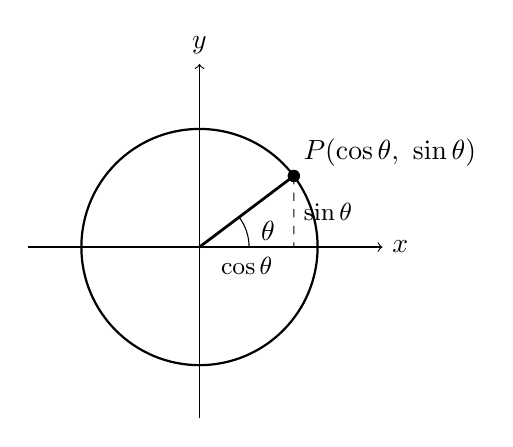
\begin{tikzpicture}[scale=1.5]
  \draw[->] (-1.45,0) -- (1.55,0) node[right] {$x$};
  \draw[->] (0,-1.45) -- (0,1.55) node[above] {$y$};
  \draw[line width=0.8pt] (0,0) circle (1);
  \coordinate (P) at (37:1);
  \draw[line width=1pt] (0,0) -- (P);
  \draw[dashed] (P) -- (37:1 |- 0,0);
  \fill (P) circle (1.5pt);
  \node[above right] at (P) {$P(\cos\theta,\ \sin\theta)$};
  \draw (0.42,0) arc (0:37:0.42);
  \node at (0.58,0.14) {$\theta$};
  \node[below] at (0.4,0) {\small $\cos\theta$};
  \node[right] at (0.8,0.3) {\small $\sin\theta$};
\end{tikzpicture}
\end{center}

\noindent
\textbf{পুরোনো সংজ্ঞার সঙ্গে মিল : } $\theta$ সূক্ষ্মকোণ হলে $P$ পড়ে প্রথম
quadrant-এ। $P$ থেকে $x$-অক্ষে লম্ব ফেললে একটি সমকোণী ত্রিভুজ পাই যার অতিভুজ
$1$ (ব্যাসার্ধ), ভূমি $x$ আর লম্ব $y$। প্রথম অনুচ্ছেদের সংজ্ঞা অনুযায়ী তখন
\[
  \sin\theta = \frac{y}{1} = y, \qquad \cos\theta = \frac{x}{1} = x ,
\]
যা ঠিক নতুন সংজ্ঞাটিই। অর্থাৎ নতুন সংজ্ঞা পুরোনোটিকে বাতিল করছে না, কেবল
বাড়িয়ে দিচ্ছে।

ব্যাসার্ধ $1$ না হয়ে $r$ হলেও কিছু বদলায় না: সদৃশ ত্রিভুজের যুক্তিতে
$\sin\theta = y/r$ এবং $\cos\theta = x/r$।

\begin{idea}[চিহ্ন কোন quadrant-এ কী]
$\cos\theta$ হলো $P$-এর $x$-স্থানাঙ্ক আর $\sin\theta$ হলো $y$-স্থানাঙ্ক, তাই
চিহ্ন মনে রাখার আলাদা কিছু নেই; quadrant-এর চিহ্নই যথেষ্ট।

প্রথম quadrant-এ দুটিই ধনাত্মক। দ্বিতীয়তে $x<0, y>0$, তাই কেবল $\sin$
ধনাত্মক। তৃতীয়তে দুটিই ঋণাত্মক, তাই তাদের ভাগফল $\tan$ ধনাত্মক। চতুর্থে
$x>0, y<0$, তাই কেবল $\cos$ ধনাত্মক।
\end{idea}

\begin{example}
$\theta = \dfrac{4\pi}{3}$-এর জন্য $\sin$, $\cos$ ও $\tan$-এর সঠিক মান বের করো।
\end{example}

\begin{solbox}
$\dfrac{4\pi}{3} = 240^\circ$, তাই $P$ তৃতীয় quadrant-এ। $x$-অক্ষ থেকে তার
কৌণিক দূরত্ব $240^\circ - 180^\circ = 60^\circ$, অর্থাৎ $\pi/3$।

$60^\circ$-এর মান আমরা জানি: $\cos 60^\circ = \tfrac{1}{2}$,
$\sin 60^\circ = \tfrac{\sqrt{3}}{2}$। তৃতীয় quadrant-এ দুটি স্থানাঙ্কই
ঋণাত্মক, তাই
\[
  \cos \frac{4\pi}{3} = -\frac{1}{2}, \qquad
  \sin \frac{4\pi}{3} = -\frac{\sqrt{3}}{2}, \qquad
  \tan \frac{4\pi}{3} = \frac{-\sqrt{3}/2}{-1/2} = \sqrt{3} .
\]
\end{solbox}

\begin{remark}
এখন অধ্যায় ৪-এর ভাষায় কথাটা গুছিয়ে বলা যায়, আর সেটাই এই অনুচ্ছেদের আসল
অর্জন। প্রান্তিক বাহু যেকোনো বাস্তব $\theta$-এর জন্যই আঁকা যায়, তাই
\[
  \sin \colon \mathbb{R} \to [-1, 1], \qquad
  \cos \colon \mathbb{R} \to [-1, 1] .
\]
Domain গোটা $\mathbb{R}$, আর range $[-1,1]$, কারণ একক বৃত্তের কোনো বিন্দুর
স্থানাঙ্ক $1$ ছাড়াতে পারে না। দুটিই surjective কিন্তু কোনোটিই injective নয়।

আরও একটি জিনিস ছবি থেকেই পড়ে নেওয়া যায়: $\theta$-এর সঙ্গে $2\pi$ যোগ করলে
প্রান্তিক বাহু একবার পুরো ঘুরে ঠিক আগের জায়গায় ফেরে, তাই
\[
  \sin(\theta + 2\pi) = \sin\theta, \qquad \cos(\theta + 2\pi) = \cos\theta .
\]
একেই বলে পর্যায়বৃত্ততা, আর $2\pi$ হলো পর্যায়কাল। পদার্থবিজ্ঞানে যত কিছু
দোলে বা ঘোরে, সবই শেষ পর্যন্ত এই দুটি ফাংশনের ভাষায় লেখা হয়।
\end{remark}

% ============================================================================
\section{মৌলিক অভেদ}
% ============================================================================

\begin{idea}[পিথাগোরীয় অভেদ]
সব বাস্তব $\theta$-এর জন্য
\[
  \sin^2\theta + \cos^2\theta = 1 .
\]
\end{idea}

\noindent
\textbf{প্রমাণ।} $P(\cos\theta, \sin\theta)$ বিন্দুটি একক বৃত্তের উপর, আর
অধ্যায় ৬ অনুযায়ী ওই বৃত্তের সমীকরণ $x^2 + y^2 = 1$। বিন্দুটির স্থানাঙ্ক
বসিয়ে দিলেই ফলটি পাওয়া যায়। $\blacksquare$

প্রথম অনুচ্ছেদের ত্রিভুজে এটি ছিল স্রেফ পিথাগোরাস, আর এখানে সেটি বৃত্তের
সমীকরণ; দুটি আসলে একই কথা, কারণ বৃত্তের সমীকরণটিও পিথাগোরাস থেকেই এসেছিল।

\begin{idea}[আরও দুটি রূপ]
$\sin^2\theta + \cos^2\theta = 1$-কে $\cos^2\theta$ দিয়ে ভাগ করলে
\[
  \tan^2\theta + 1 = \sec^2\theta ,
\]
আর $\sin^2\theta$ দিয়ে ভাগ করলে
\[
  1 + \cot^2\theta = \csc^2\theta .
\]
প্রথমটির জন্য $\cos\theta \neq 0$ আর দ্বিতীয়টির জন্য $\sin\theta \neq 0$ লাগবে,
যা ওই ফাংশনগুলোর সংজ্ঞা থেকেই এমনিতেই ধরা আছে।
\end{idea}

\begin{idea}[জোড়, বিজোড় ও পূরক কোণ]
সব $\theta$-এর জন্য
\[
  \sin(-\theta) = -\sin\theta, \qquad \cos(-\theta) = \cos\theta ,
\]
\[
  \sin\!\left( \frac{\pi}{2} - \theta \right) = \cos\theta, \qquad
  \cos\!\left( \frac{\pi}{2} - \theta \right) = \sin\theta .
\]
অর্থাৎ $\sin$ একটি বিজোড় function আর $\cos$ একটি জোড় function।
\end{idea}

\noindent
\textbf{প্রমাণ।} প্রথম জোড়ার জন্য: $\theta$-এর বদলে $-\theta$ নেওয়া মানে
প্রান্তিক বাহুটিকে উল্টো দিকে ঘোরানো, যা $P$ বিন্দুটিকে $x$-অক্ষের সাপেক্ষে
প্রতিফলিত করে। প্রতিফলনে $x$-স্থানাঙ্ক অপরিবর্তিত থাকে আর $y$-স্থানাঙ্ক চিহ্ন
বদলায়, তাই $\cos$ একই থাকে আর $\sin$-এর চিহ্ন বদলায়।

দ্বিতীয় জোড়ার জন্য: দাবি করি $(a,b)$ বিন্দুর $y = x$ রেখার সাপেক্ষে প্রতিফলন
হলো $(b,a)$। কারণ দুটি বিন্দুর সংযোজক রেখাংশের মধ্যবিন্দু
$\left( \tfrac{a+b}{2}, \tfrac{a+b}{2} \right)$, যা $y=x$ রেখার উপরেই আছে; আর
ওই রেখাংশের ঢাল $\dfrac{a-b}{b-a} = -1$, যা $y=x$ রেখার ঢাল $1$-এর সঙ্গে গুণ
করলে $-1$ দেয়, অর্থাৎ লম্ব (অধ্যায় ৬)। মধ্যবিন্দু রেখার উপর এবং সংযোজক
রেখাংশ রেখার উপর লম্ব, তাই এটিই প্রতিফলন।

এখন $y=x$ রেখাটি $x$-অক্ষের সঙ্গে $\pi/4$ কোণ করে, তাই এর সাপেক্ষে প্রতিফলন
$\theta$ কোণকে পাঠায় $2 \cdot \dfrac{\pi}{4} - \theta = \dfrac{\pi}{2} - \theta$
কোণে। সুতরাং $\left( \cos\theta, \sin\theta \right)$-এর প্রতিফলন একদিকে
$\left( \sin\theta, \cos\theta \right)$, আর অন্যদিকে সেটিই
$\dfrac{\pi}{2} - \theta$ কোণের বিন্দু, অর্থাৎ
$\left( \cos\!\left( \tfrac{\pi}{2} - \theta \right),
\sin\!\left( \tfrac{\pi}{2} - \theta \right) \right)$। স্থানাঙ্ক মিলিয়ে দিলেই
দাবি দুটি পাওয়া যায়। $\blacksquare$

\begin{example}
প্রমাণ করো: $\ \tan^2\theta - \sin^2\theta = \tan^2\theta \, \sin^2\theta$।
\end{example}

\begin{solbox}
অভেদ প্রমাণের সাধারণ কৌশল হলো এক পাশ ধরে সব কিছু $\sin$ ও $\cos$-এ নামিয়ে আনা।
বাঁ পাশ নিই:
\[
  \tan^2\theta - \sin^2\theta
  = \frac{\sin^2\theta}{\cos^2\theta} - \sin^2\theta
  = \sin^2\theta \left( \frac{1}{\cos^2\theta} - 1 \right)
  = \sin^2\theta \cdot \frac{1 - \cos^2\theta}{\cos^2\theta} .
\]
পিথাগোরীয় অভেদে $1 - \cos^2\theta = \sin^2\theta$, তাই এটি দাঁড়ায়
\[
  \sin^2\theta \cdot \frac{\sin^2\theta}{\cos^2\theta}
  = \sin^2\theta \, \tan^2\theta ,
\]
যা ডান পাশ। $\blacksquare$
\end{solbox}

% ============================================================================
\section{যোগ ও বিয়োগ সূত্র}
% ============================================================================

এই অনুচ্ছেদটিই অধ্যায়ের কেন্দ্র। একটিমাত্র সূত্র প্রমাণ করা হবে, আর বাকি
সবগুলো তার থেকে বেরিয়ে আসবে।

\begin{idea}[বিয়োগ সূত্র]
সব বাস্তব $\alpha, \beta$-এর জন্য
\[
  \cos(\alpha - \beta) = \cos\alpha \cos\beta + \sin\alpha \sin\beta .
\]
\end{idea}

\noindent
\textbf{প্রমাণ।} কৌশলটি হলো একটি দৈর্ঘ্য দুইভাবে হিসাব করা।

একক বৃত্তের উপর দুটি বিন্দু নাও:
\[
  A = (\cos\alpha,\ \sin\alpha), \qquad B = (\cos\beta,\ \sin\beta) .
\]
অধ্যায় ৬-এর দূরত্ব সূত্রে
\[
  |AB|^2 = (\cos\alpha - \cos\beta)^2 + (\sin\alpha - \sin\beta)^2 .
\]
বর্গ খুলে লিখি:
\[
  |AB|^2 = \cos^2\alpha - 2\cos\alpha\cos\beta + \cos^2\beta
         + \sin^2\alpha - 2\sin\alpha\sin\beta + \sin^2\beta .
\]
$\cos^2\alpha + \sin^2\alpha = 1$ এবং $\cos^2\beta + \sin^2\beta = 1$, তাই
\[
  |AB|^2 = 2 - 2\big( \cos\alpha\cos\beta + \sin\alpha\sin\beta \big) . \tag{i}
\]

এবার একই দৈর্ঘ্য অন্যভাবে। বৃত্তের উপর আরও দুটি বিন্দু নাও:
\[
  P = (1,\ 0), \qquad Q = \big( \cos(\alpha - \beta),\ \sin(\alpha-\beta) \big) .
\]
একই দূরত্ব সূত্রে
\[
  |PQ|^2 = \big( \cos(\alpha-\beta) - 1 \big)^2 + \sin^2(\alpha-\beta)
         = 2 - 2\cos(\alpha - \beta) . \tag{ii}
\]

দাবি: $|AB| = |PQ|$। কারণ $OA$, $OB$, $OP$, $OQ$ প্রতিটিই ব্যাসার্ধ, অর্থাৎ
দৈর্ঘ্য $1$; আর $AOB$ কোণটি দুই বাহুর দিকের পার্থক্য, অর্থাৎ $\alpha - \beta$,
ঠিক যেমন $POQ$ কোণটিও গড়ন অনুযায়ী $\alpha - \beta$। দুই বাহু ও তাদের
অন্তর্ভুক্ত কোণ সমান, তাই ত্রিভুজ $OAB$ ও $OPQ$ সর্বসম (অধ্যায় ৫), ফলে
তৃতীয় বাহু দুটিও সমান।

(i) ও (ii) সমান বসিয়ে দিলে
\[
  2 - 2\cos(\alpha-\beta) = 2 - 2\big( \cos\alpha\cos\beta + \sin\alpha\sin\beta \big),
\]
আর দুই পাশ থেকে $2$ বাদ দিয়ে $-2$ দিয়ে ভাগ করলেই ফলটি পাওয়া যায়।
$\blacksquare$

\begin{center}
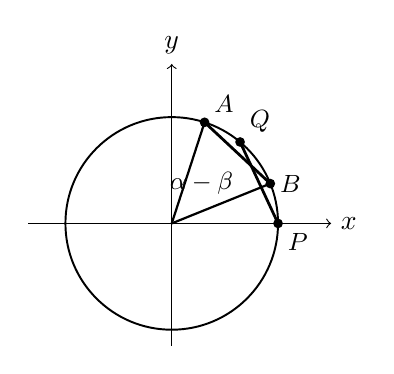
\begin{tikzpicture}[scale=1.35]
  \draw[->] (-1.35,0) -- (1.5,0) node[right] {$x$};
  \draw[->] (0,-1.15) -- (0,1.5) node[above] {$y$};
  \draw[line width=0.7pt] (0,0) circle (1);
  \coordinate (A) at (72:1);
  \coordinate (B) at (22:1);
  \coordinate (P) at (0:1);
  \coordinate (Q) at (50:1);
  \draw[line width=0.8pt] (0,0) -- (A);
  \draw[line width=0.8pt] (0,0) -- (B);
  \draw[line width=1pt] (A) -- (B);
  \draw[line width=1pt] (P) -- (Q);
  \fill (A) circle (1.3pt) node[above right] {\small $A$};
  \fill (B) circle (1.3pt) node[right] {\small $B$};
  \fill (P) circle (1.3pt) node[below right] {\small $P$};
  \fill (Q) circle (1.3pt) node[above right] {\small $Q$};
  \node at (0.28,0.38) {\small $\alpha-\beta$};
\end{tikzpicture}
\end{center}

\noindent
ছবিতে $AB$ ও $PQ$ জ্যা দুটির দৈর্ঘ্য সমান, কারণ দুটিই একই বৃত্তে একই পরিমাণ
কেন্দ্রস্থ কোণ কাটে।

\begin{idea}[বাকি তিনটি]
উপরের একটি সূত্র থেকে বাকিগুলো:
\[
  \cos(\alpha + \beta) = \cos\alpha\cos\beta - \sin\alpha\sin\beta ,
\]
\[
  \sin(\alpha + \beta) = \sin\alpha\cos\beta + \cos\alpha\sin\beta ,
\]
\[
  \sin(\alpha - \beta) = \sin\alpha\cos\beta - \cos\alpha\sin\beta .
\]
\end{idea}

\noindent
\textbf{উৎপত্তি।} প্রথমটির জন্য বিয়োগ সূত্রে $\beta$-এর জায়গায় $-\beta$ বসাও,
আর জোড়-বিজোড় অভেদ ব্যবহার করো:
\[
  \cos(\alpha + \beta) = \cos\big( \alpha - (-\beta) \big)
  = \cos\alpha\cos(-\beta) + \sin\alpha\sin(-\beta)
  = \cos\alpha\cos\beta - \sin\alpha\sin\beta .
\]

দ্বিতীয়টির জন্য পূরক কোণের অভেদ দিয়ে $\sin$-কে $\cos$-এ অনুবাদ করি:
\[
  \sin(\alpha+\beta) = \cos\!\left( \frac{\pi}{2} - \alpha - \beta \right)
  = \cos\!\left( \Big( \frac{\pi}{2} - \alpha \Big) - \beta \right) .
\]
এবার বিয়োগ সূত্র প্রয়োগ করে
\[
  = \cos\!\left( \frac{\pi}{2} - \alpha \right)\cos\beta
  + \sin\!\left( \frac{\pi}{2} - \alpha \right)\sin\beta
  = \sin\alpha\cos\beta + \cos\alpha\sin\beta .
\]

তৃতীয়টির জন্য দ্বিতীয়টিতে $\beta$-এর বদলে $-\beta$ বসাও। $\blacksquare$

\begin{idea}[tangent ও দ্বিগুণ কোণ]
যোগ সূত্র দুটিকে ভাগ করে, লব ও হরকে $\cos\alpha\cos\beta$ দিয়ে ভাগ করলে
\[
  \tan(\alpha \pm \beta) = \frac{\tan\alpha \pm \tan\beta}
                                {1 \mp \tan\alpha\tan\beta} .
\]
আর যোগ সূত্রে $\beta = \alpha$ বসালে দ্বিগুণ কোণের সূত্র:
\[
  \sin 2\alpha = 2\sin\alpha\cos\alpha, \qquad
  \cos 2\alpha = \cos^2\alpha - \sin^2\alpha .
\]
পিথাগোরীয় অভেদ খাটিয়ে দ্বিতীয়টির আরও দুটি রূপ পাওয়া যায়:
\[
  \cos 2\alpha = 2\cos^2\alpha - 1 = 1 - 2\sin^2\alpha .
\]
\end{idea}

\begin{example}
$\cos 15^\circ$-এর সঠিক মান বের করো।
\end{example}

\begin{solbox}
$15^\circ$ সরাসরি চেনা কোণ নয়, কিন্তু $15^\circ = 45^\circ - 30^\circ$, আর
দুটিই চেনা। বিয়োগ সূত্রে
\[
  \cos 15^\circ = \cos 45^\circ \cos 30^\circ + \sin 45^\circ \sin 30^\circ
  = \frac{1}{\sqrt{2}} \cdot \frac{\sqrt{3}}{2}
  + \frac{1}{\sqrt{2}} \cdot \frac{1}{2}
  = \frac{\sqrt{3} + 1}{2\sqrt{2}} .
\]
হর মূলদ করে
\[
  \cos 15^\circ = \frac{(\sqrt{3}+1)\sqrt{2}}{4} = \frac{\sqrt{6} + \sqrt{2}}{4} .
\]
মান আনুমানিক $0.9659$, যা যুক্তিসঙ্গত: $15^\circ$ ছোট কোণ, তাই $\cos$ $1$-এর
কাছাকাছি থাকারই কথা।
\end{solbox}

\begin{remark}
শেষ বাক্যটিতে যা করা হলো, সেটা নিছক যাচাই নয়; ওখানেই একটা বড় ধারণার বীজ আছে।
কোণ ছোট হলে $\cos\theta$ প্রায় $1$ আর $\sin\theta$ প্রায় $\theta$ হয়ে যায়,
আর পদার্থবিজ্ঞানে এই আসন্নীকরণটি সম্ভবত সবচেয়ে বেশি ব্যবহৃত আসন্নীকরণ; দোলক
থেকে আলোকবিজ্ঞান, সর্বত্র। অধ্যায় ১৩-এ একক বৃত্ত থেকেই এটি জ্যামিতিকভাবে
প্রতিষ্ঠা করা হবে।

তবে ``প্রায়'' কথাটার সঠিক মানে কী, আর ভুলটা ঠিক কত বড়, সেই প্রশ্নের উত্তর
ত্রিকোণমিতি দিতে পারে না; তার জন্য derivative লাগে। অধ্যায় ১৫-এ Taylor
সিরিজ দিয়ে $\sin\theta \approx \theta$ আর
$\cos\theta \approx 1 - \theta^2/2$ যথাযথভাবে বের করা হবে, আর তখন আজকের এই
আন্দাজটা একটা প্রমাণে পরিণত হবে।
\end{remark}

% ============================================================================
\section{বাস্তব প্রয়োগ}
% ============================================================================

এতক্ষণ কোণ ছিল একক বৃত্তে। এবার আবার ত্রিভুজে ফিরি, তবে এবার আর সমকোণ লাগবে না।

\begin{idea}[ত্রিভুজের ক্ষেত্রফল]
কোনো ত্রিভুজের দুটি বাহু $a$ ও $b$, আর তাদের অন্তর্ভুক্ত কোণ $C$ হলে
\[
  \text{ক্ষেত্রফল} = \tfrac{1}{2}\, a b \sin C .
\]
\end{idea}

\noindent
\textbf{উৎপত্তি।} $b$ বাহুটিকে ভূমি ধরো। $a$ বাহুর অপর প্রান্ত থেকে ভূমির উপর
লম্ব ফেললে যে উচ্চতা $h$ পাই, সেই লম্ব একটি সমকোণী ত্রিভুজ তৈরি করে যার অতিভুজ
$a$ আর $C$-এর বিপরীত বাহু $h$। তাই $h = a \sin C$, এবং
\[
  \text{ক্ষেত্রফল} = \tfrac{1}{2} \times \text{ভূমি} \times \text{উচ্চতা}
  = \tfrac{1}{2} b \cdot a \sin C .
\]
$C$ স্থূলকোণ হলে লম্বের পাদবিন্দু ভূমির বাইরে পড়ে, কিন্তু উচ্চতা তখনো
$a \sin C$ থাকে এবং $0 < C < \pi$ বলে $\sin C > 0$; তাই সূত্রটি অটুট।
$\blacksquare$

\begin{idea}[সাইন সূত্র]
যেকোনো ত্রিভুজে, বাহুগুলো $a, b, c$ আর তাদের বিপরীত কোণ $A, B, C$ হলে
\[
  \frac{a}{\sin A} = \frac{b}{\sin B} = \frac{c}{\sin C} .
\]
\end{idea}

\noindent
\textbf{উৎপত্তি।} একই ত্রিভুজের ক্ষেত্রফল তিনভাবে লেখা যায়, কোন জোড়া বাহু
বেছে নিচ্ছি তার উপর নির্ভর করে:
\[
  \tfrac{1}{2} ab \sin C = \tfrac{1}{2} bc \sin A = \tfrac{1}{2} ca \sin B .
\]
তিনটিকেই $\tfrac{1}{2}abc$ দিয়ে ভাগ করলে
\[
  \frac{\sin C}{c} = \frac{\sin A}{a} = \frac{\sin B}{b} ,
\]
আর উল্টে নিলেই কাঙ্ক্ষিত রূপ। $\blacksquare$

\begin{idea}[কোসাইন সূত্র]
একই বর্ণনায়,
\[
  c^2 = a^2 + b^2 - 2ab\cos C .
\]
\end{idea}

\noindent
\textbf{উৎপত্তি।} স্থানাঙ্ক বসিয়ে দিলেই হয়ে যায়। $C$ কোণটিকে আদর্শ অবস্থানে
রাখো: শীর্ষ origin-এ, আর $a$ বাহুটি ধনাত্মক $x$-অক্ষ বরাবর, তাই তার অপর প্রান্ত
$(a, 0)$। অন্য বাহুটির দৈর্ঘ্য $b$ এবং সে $x$-অক্ষের সঙ্গে $C$ কোণ করে, তাই তার
অপর প্রান্ত $(b\cos C,\ b\sin C)$।

$c$ হলো এই দুই প্রান্তের দূরত্ব, তাই অধ্যায় ৬-এর সূত্রে
\[
  c^2 = (b\cos C - a)^2 + (b \sin C)^2
      = b^2\cos^2 C - 2ab\cos C + a^2 + b^2 \sin^2 C .
\]
$b^2(\cos^2 C + \sin^2 C) = b^2$, সুতরাং
$c^2 = a^2 + b^2 - 2ab\cos C$. $\blacksquare$

\begin{remark}
$C = \dfrac{\pi}{2}$ বসাও: $\cos C = 0$, আর সূত্রটি দাঁড়ায় $c^2 = a^2 + b^2$।
অর্থাৎ কোসাইন সূত্র পিথাগোরাসেরই সাধারণ রূপ, আর $-2ab\cos C$ পদটি হলো সমকোণ
থেকে সরে যাওয়ার জরিমানা। কোণ সূক্ষ্ম হলে $\cos C > 0$, তাই $c$ ছোট হয়; স্থূল
হলে $\cos C < 0$, তাই $c$ বড় হয়। ছবি না এঁকেও এটা ঠিক মনে হয়।
\end{remark}

\begin{example}
একটি ত্রিভুজের দুটি বাহু $8$ ও $5$ একক, আর তাদের অন্তর্ভুক্ত কোণ $60^\circ$।
তৃতীয় বাহুটি বের করো।
\end{example}

\begin{solbox}
কোসাইন সূত্রে $a = 8$, $b = 5$, $C = 60^\circ$, আর $\cos 60^\circ = \tfrac{1}{2}$:
\[
  c^2 = 8^2 + 5^2 - 2 \cdot 8 \cdot 5 \cdot \tfrac{1}{2}
      = 64 + 25 - 40 = 49 ,
\]
তাই $c = 7$।
\end{solbox}

\begin{example}
একটি খাড়া টাওয়ারের পাদদেশের দিকে মুখ করে সমতল মাঠে দুটি বিন্দু $P$ ও $Q$ একই
সরলরেখায় আছে, $PQ = 40$ মিটার, আর $Q$ টাওয়ারের কাছে। $P$ থেকে চূড়ার উন্নতি কোণ
$30^\circ$ এবং $Q$ থেকে $45^\circ$। টাওয়ারের উচ্চতা বের করো।
\end{example}

\begin{solbox}
উচ্চতা $h$, আর টাওয়ারের পাদদেশ থেকে $Q$-এর দূরত্ব $d$ ধরি। দুটি সমকোণী ত্রিভুজ
পাই, দুটিরই উল্লম্ব বাহু $h$।

$Q$ থেকে: $\tan 45^\circ = \dfrac{h}{d}$, আর $\tan 45^\circ = 1$, তাই $d = h$।

$P$ থেকে: $\tan 30^\circ = \dfrac{h}{d + 40}$, আর
$\tan 30^\circ = \dfrac{1}{\sqrt{3}}$, তাই $d + 40 = h\sqrt{3}$।

প্রথমটি দ্বিতীয়টিতে বসিয়ে
\[
  h + 40 = h\sqrt{3}
  \ \Longrightarrow\ h(\sqrt{3} - 1) = 40
  \ \Longrightarrow\ h = \frac{40}{\sqrt{3}-1} .
\]
হর মূলদ করে
\[
  h = \frac{40(\sqrt{3}+1)}{(\sqrt{3}-1)(\sqrt{3}+1)} = \frac{40(\sqrt{3}+1)}{2}
    = 20(\sqrt{3}+1) \approx 54.6 \text{ মিটার} .
\]
\end{solbox}

\begin{remark}
শেষ একটি প্রয়োগ, যা এই সিরিজের আসল গন্তব্যের দিকে ইশারা করে। অনুভূমিকের সঙ্গে
$\theta$ কোণে $v_0$ দ্রুতিতে ছোঁড়া একটি বস্তুর অনুভূমিক পাল্লা (মাটিতে পড়ার পূর্বে পর্যন্ত মাটি বরাবর যে দূরত্ব অতিক্রম করে)
\[
  R = \frac{v_0^2 \sin 2\theta}{g} .
\]
এই সূত্রটি এখানে প্রমাণ করা হয়নি; এটি গতিবিদ্যা থেকে ধার করা, আর এই সিরিজে
তার জায়গা এখনো আসেনি। কিন্তু সূত্রটি মেনে নিলে ত্রিকোণমিতি বাকি কাজটা এক
লাইনে সেরে দেয়।

$\sin$-এর সর্বোচ্চ মান $1$, আর $0 < \theta < 90^\circ$ পরিসরে $\sin 2\theta = 1$
হয় কেবল $2\theta = 90^\circ$, অর্থাৎ $\theta = 45^\circ$-এ। তাই পাল্লা সবচেয়ে
বেশি হয় $45^\circ$ কোণে। কোনো calculus লাগল না, কেবল range-এর কথাটা জানলেই হলো।

আরও একটি জিনিস বেরিয়ে আসে। বিয়োগ সূত্রে $\sin(180^\circ - x) = \sin x$, তাই
$\theta$ আর $90^\circ - \theta$ ঠিক একই পাল্লা দেয়। $30^\circ$ ও $60^\circ$
কোণে ছোঁড়া দুটি বল একই জায়গায় পড়ে, যদিও একটি অনেক উঁচুতে ওঠে আর অনেক বেশি
সময় নেয়।
\end{remark}

% ============================================================================
\section{সমস্যা}
% ============================================================================

\prob{1} রূপান্তর করো।
\begin{enumerate}
  \item $210^\circ$ ও $-135^\circ$ কে radian-এ।
  \item $\dfrac{5\pi}{12}$ ও $\dfrac{11\pi}{6}$ radian কে degree-তে।
\end{enumerate}

\begin{sol}
\begin{enumerate}
  \item $210 \times \dfrac{\pi}{180} = \dfrac{7\pi}{6}$ এবং
        $-135 \times \dfrac{\pi}{180} = -\dfrac{3\pi}{4}$।
  \item $\dfrac{5\pi}{12} \times \dfrac{180}{\pi} = 75^\circ$ এবং
        $\dfrac{11\pi}{6} \times \dfrac{180}{\pi} = 330^\circ$।
\end{enumerate}
\end{sol}

\prob{1} একটি বৃত্তের ব্যাসার্ধ $12$ cm।
\begin{enumerate}
  \item $\dfrac{2\pi}{3}$ radian কেন্দ্রস্থ কোণ কত দৈর্ঘ্যের চাপ কাটে?
  \item $9$ cm দৈর্ঘ্যের একটি চাপ কেন্দ্রে কত radian কোণ ধারণ করে?
\end{enumerate}

\begin{sol}
\begin{enumerate}
  \item $s = r\theta = 12 \times \dfrac{2\pi}{3} = 8\pi$ cm।
  \item $\theta = \dfrac{s}{r} = \dfrac{9}{12} = 0.75$ radian।
\end{enumerate}
\end{sol}

\prob{2} $\theta = \dfrac{5\pi}{6}$ এবং $\theta = \dfrac{7\pi}{4}$-এর জন্য
$\sin\theta$, $\cos\theta$ ও $\tan\theta$-এর সঠিক মান বের করো।

\begin{sol}
$\dfrac{5\pi}{6} = 150^\circ$, দ্বিতীয় quadrant, $x$-অক্ষ থেকে কৌণিক দূরত্ব
$30^\circ$। দ্বিতীয় quadrant-এ $\sin$ ধনাত্মক, $\cos$ ঋণাত্মক:
\[
  \sin\frac{5\pi}{6} = \frac{1}{2}, \qquad
  \cos\frac{5\pi}{6} = -\frac{\sqrt{3}}{2}, \qquad
  \tan\frac{5\pi}{6} = -\frac{1}{\sqrt{3}} .
\]

$\dfrac{7\pi}{4} = 315^\circ$, চতুর্থ quadrant, কৌণিক দূরত্ব $45^\circ$।
চতুর্থ quadrant-এ $\cos$ ধনাত্মক, $\sin$ ঋণাত্মক:
\[
  \sin\frac{7\pi}{4} = -\frac{1}{\sqrt{2}}, \qquad
  \cos\frac{7\pi}{4} = \frac{1}{\sqrt{2}}, \qquad
  \tan\frac{7\pi}{4} = -1 .
\]
\end{sol}

\prob{2} $\cos\theta = -\dfrac{3}{5}$ এবং $\dfrac{\pi}{2} < \theta < \pi$ হলে
বাকি পাঁচটি অনুপাত বের করো।

\begin{sol}
পিথাগোরীয় অভেদে
$\sin^2\theta = 1 - \dfrac{9}{25} = \dfrac{16}{25}$, তাই
$\sin\theta = \pm\dfrac{4}{5}$। $\theta$ দ্বিতীয় quadrant-এ, সেখানে $\sin$
ধনাত্মক, তাই $\sin\theta = \dfrac{4}{5}$।

বাকিগুলো সংজ্ঞা থেকেই:
\[
  \tan\theta = \frac{4/5}{-3/5} = -\frac{4}{3}, \qquad
  \cot\theta = -\frac{3}{4}, \qquad
  \sec\theta = -\frac{5}{3}, \qquad
  \csc\theta = \frac{5}{4} .
\]
চিহ্নগুলো মিলিয়ে দেখো: দ্বিতীয় quadrant-এ কেবল $\sin$ ও $\csc$ ধনাত্মক, আর
ঠিক তাই হয়েছে।
\end{sol}

\prob{2} প্রমাণ করো:
$\ \dfrac{1}{1 - \sin\theta} + \dfrac{1}{1 + \sin\theta} = 2\sec^2\theta$।

\begin{sol}
বাঁ পাশের দুটি ভগ্নাংশ যোগ করি:
\[
  \frac{(1 + \sin\theta) + (1 - \sin\theta)}{(1 - \sin\theta)(1 + \sin\theta)}
  = \frac{2}{1 - \sin^2\theta} .
\]
পিথাগোরীয় অভেদে হর $= \cos^2\theta$, তাই এটি
$\dfrac{2}{\cos^2\theta} = 2\sec^2\theta$, যা ডান পাশ।
$\sin\theta = \pm 1$ হলে বাঁ পাশ সংজ্ঞায়িত নয়, আর ঠিক তখনই $\cos\theta = 0$
হয়ে ডান পাশও সংজ্ঞায়িত থাকে না; তাই দুই পাশের domain এক।
\end{sol}

\prob{2} প্রমাণ করো: $\ \sec\theta - \cos\theta = \tan\theta \sin\theta$।

\begin{sol}
বাঁ পাশ:
\[
  \frac{1}{\cos\theta} - \cos\theta
  = \frac{1 - \cos^2\theta}{\cos\theta}
  = \frac{\sin^2\theta}{\cos\theta}
  = \frac{\sin\theta}{\cos\theta} \cdot \sin\theta
  = \tan\theta \sin\theta . \qquad \blacksquare
\]
\end{sol}

\prob{2} একটি খাড়া পাহাড়ের চূড়া সমুদ্রপৃষ্ঠ থেকে $25$ মিটার উঁচু। চূড়া থেকে
একটি নৌকার অবনতি কোণ $30^\circ$। নৌকাটি পাহাড়ের পাদদেশ থেকে কত দূরে?

\begin{sol}
অবনতি কোণ $30^\circ$ মানে নৌকা থেকে চূড়ার উন্নতি কোণও $30^\circ$, কারণ
অনুভূমিক রেখা দুটি সমান্তরাল আর এরা একান্তর কোণ (অধ্যায় ৫)।

দূরত্ব $d$ ধরে, সমকোণী ত্রিভুজে
\[
  \tan 30^\circ = \frac{25}{d}
  \ \Longrightarrow\ \frac{1}{\sqrt{3}} = \frac{25}{d}
  \ \Longrightarrow\ d = 25\sqrt{3} \approx 43.3 \text{ মিটার} .
\]
\end{sol}

\prob{2} $\sin 75^\circ$-এর সঠিক মান বের করো।

\begin{sol}
$75^\circ = 45^\circ + 30^\circ$, তাই যোগ সূত্রে
\[
  \sin 75^\circ = \sin 45^\circ \cos 30^\circ + \cos 45^\circ \sin 30^\circ
  = \frac{1}{\sqrt{2}} \cdot \frac{\sqrt{3}}{2}
  + \frac{1}{\sqrt{2}} \cdot \frac{1}{2}
  = \frac{\sqrt{3}+1}{2\sqrt{2}} = \frac{\sqrt{6}+\sqrt{2}}{4} .
\]
লক্ষ করো এটি $\cos 15^\circ$-এর সমান, যা প্রত্যাশিত, কারণ
$75^\circ$ ও $15^\circ$ পূরক কোণ।
\end{sol}

\prob{3} $\sin x = \dfrac{3}{5}$ যেখানে $0 < x < \dfrac{\pi}{2}$, এবং
$\cos y = -\dfrac{5}{13}$ যেখানে $\dfrac{\pi}{2} < y < \pi$। নিচেরগুলো বের করো।
\begin{enumerate}
  \item $\sin(x+y)$
  \item $\cos(x-y)$
  \item $\sin 2y$
\end{enumerate}

\begin{sol}
প্রথমে অজানা দুটি বের করি। $x$ প্রথম quadrant-এ, তাই
$\cos x = +\sqrt{1 - \tfrac{9}{25}} = \dfrac{4}{5}$।
$y$ দ্বিতীয় quadrant-এ, তাই
$\sin y = +\sqrt{1 - \tfrac{25}{169}} = \dfrac{12}{13}$।

\begin{enumerate}
  \item
        \[
          \sin(x+y) = \sin x \cos y + \cos x \sin y
          = \frac{3}{5}\cdot\left(-\frac{5}{13}\right)
          + \frac{4}{5}\cdot\frac{12}{13}
          = \frac{-15 + 48}{65} = \frac{33}{65} .
        \]
  \item
        \[
          \cos(x-y) = \cos x \cos y + \sin x \sin y
          = \frac{4}{5}\cdot\left(-\frac{5}{13}\right)
          + \frac{3}{5}\cdot\frac{12}{13}
          = \frac{-20 + 36}{65} = \frac{16}{65} .
        \]
  \item
        \[
          \sin 2y = 2 \sin y \cos y
          = 2 \cdot \frac{12}{13} \cdot \left(-\frac{5}{13}\right)
          = -\frac{120}{169} .
        \]
        ঋণাত্মক হওয়াই স্বাভাবিক: $\dfrac{\pi}{2} < y < \pi$ হলে
        $\pi < 2y < 2\pi$, অর্থাৎ $2y$ নিচের অর্ধবৃত্তে, যেখানে $\sin$ ঋণাত্মক।
\end{enumerate}
\end{sol}

\prob{2} $[0, 2\pi)$ ব্যবধিতে $\sin 2x = \cos x$ সমীকরণটির সব সমাধান বের করো।

\begin{sol}
দ্বিগুণ কোণের সূত্রে বাঁ পাশ ভেঙে সব কিছু এক পাশে আনি:
\[
  2\sin x\cos x = \cos x
  \ \Longrightarrow\ \cos x\,(2\sin x - 1) = 0 .
\]
এখানে $\cos x$ দিয়ে ভাগ করা চলবে না, কারণ সে শূন্য হতে পারে; ভাগ করলে
সমাধান হারাতাম।

$\cos x = 0$ দেয় $x = \dfrac{\pi}{2}, \dfrac{3\pi}{2}$।

$\sin x = \dfrac{1}{2}$ দেয় $x = \dfrac{\pi}{6}, \dfrac{5\pi}{6}$।

চারটি সমাধান:
$\dfrac{\pi}{6}, \dfrac{\pi}{2}, \dfrac{5\pi}{6}, \dfrac{3\pi}{2}$।
\end{sol}

\prob{3} প্রমাণ করো: $\ \cos 3\theta = 4\cos^3\theta - 3\cos\theta$।

\begin{sol}
$3\theta = 2\theta + \theta$ লিখে যোগ সূত্র প্রয়োগ করি:
\[
  \cos 3\theta = \cos 2\theta \cos\theta - \sin 2\theta \sin\theta .
\]
এবার $\cos 2\theta = 2\cos^2\theta - 1$ এবং
$\sin 2\theta = 2\sin\theta\cos\theta$ বসাই:
\[
  = (2\cos^2\theta - 1)\cos\theta - 2\sin^2\theta\cos\theta
  = 2\cos^3\theta - \cos\theta - 2\cos\theta\,\sin^2\theta .
\]
শেষ পদে $\sin^2\theta = 1 - \cos^2\theta$ বসিয়ে
\[
  = 2\cos^3\theta - \cos\theta - 2\cos\theta + 2\cos^3\theta
  = 4\cos^3\theta - 3\cos\theta . \qquad \blacksquare
\]
\end{sol}

\prob{3} প্রমাণ করো:
$\ \sin^2 x - \sin^2 y = \sin(x+y)\,\sin(x-y)$।

\begin{sol}
ডান পাশ ধরে শুরু করাই সহজ, কারণ সেখানেই ভাঙার মতো জিনিস আছে:
\[
  \sin(x+y)\sin(x-y)
  = (\sin x\cos y + \cos x \sin y)(\sin x \cos y - \cos x \sin y) .
\]
এটি $(A+B)(A-B) = A^2 - B^2$ আকারের, যেখানে $A = \sin x\cos y$ এবং
$B = \cos x \sin y$। তাই
\[
  = \sin^2 x \cos^2 y - \cos^2 x \sin^2 y .
\]
এবার $\cos^2 y = 1 - \sin^2 y$ ও $\cos^2 x = 1 - \sin^2 x$ বসাই:
\[
  = \sin^2 x (1 - \sin^2 y) - (1 - \sin^2 x)\sin^2 y
  = \sin^2 x - \sin^2 x \sin^2 y - \sin^2 y + \sin^2 x \sin^2 y .
\]
মাঝের দুটি পদ কেটে যায়, থাকে $\sin^2 x - \sin^2 y$, যা বাঁ পাশ।
$\blacksquare$
\end{sol}

\prob{3} একটি ত্রিভুজের দুটি বাহু $6$ ও $10$ একক, আর তাদের অন্তর্ভুক্ত কোণ
$120^\circ$।
\begin{enumerate}
  \item তৃতীয় বাহুটি বের করো।
  \item বাকি দুটি কোণ বের করো (এক দশমিক স্থান পর্যন্ত)।
\end{enumerate}

\begin{sol}
\begin{enumerate}
  \item $a = 6$, $b = 10$, $C = 120^\circ$, আর
        $\cos 120^\circ = -\tfrac{1}{2}$। কোসাইন সূত্রে
        \[
          c^2 = 36 + 100 - 2 \cdot 6 \cdot 10 \cdot \left(-\tfrac{1}{2}\right)
              = 136 + 60 = 196 ,
        \]
        তাই $c = 14$।
  \item সাইন সূত্রে, $\sin 120^\circ = \dfrac{\sqrt{3}}{2}$ ধরে
        \[
          \sin A = \frac{a \sin C}{c} = \frac{6 \cdot \frac{\sqrt{3}}{2}}{14}
                 = \frac{3\sqrt{3}}{14} \approx 0.3712 ,
        \]
        তাই $A \approx 21.8^\circ$। এখানে স্থূলকোণ সম্ভাবনাটি বাদ, কারণ
        ত্রিভুজে ইতিমধ্যেই একটি $120^\circ$ কোণ আছে আর দুটি স্থূলকোণ থাকতে
        পারে না।

        তৃতীয় কোণ $B = 180^\circ - 120^\circ - 21.8^\circ = 38.2^\circ$।

        যাচাই: $\sin B = \dfrac{10 \cdot \frac{\sqrt{3}}{2}}{14}
        = \dfrac{5\sqrt{3}}{14} \approx 0.6186$, যা $38.2^\circ$-এর সঙ্গে
        মেলে।
\end{enumerate}
\end{sol}

\prob{3} অনুভূমিকের সঙ্গে $\theta$ কোণে $v_0$ দ্রুতিতে ছোঁড়া একটি বস্তুর
অনুভূমিক পাল্লা $R = \dfrac{v_0^2 \sin 2\theta}{g}$, যেখানে
$0 < \theta < 90^\circ$। (সূত্রটি প্রমাণ করতে হবে না; ধরে নাও।)
\begin{enumerate}
  \item দেখাও যে পাল্লা সর্বোচ্চ হয় $\theta = 45^\circ$-এ, এবং সর্বোচ্চ
        পাল্লাটি লেখো।
  \item দেখাও যে $\theta$ ও $90^\circ - \theta$ কোণ দুটি একই পাল্লা দেয়।
  \item $60^\circ$ কোণে ছোঁড়া হলে পাল্লা সর্বোচ্চ পাল্লার কত ভগ্নাংশ হবে?
\end{enumerate}

\begin{sol}
\begin{enumerate}
  \item $v_0$ ও $g$ ধ্রুবক, তাই $R$ সবচেয়ে বড় হবে যখন $\sin 2\theta$ সবচেয়ে
        বড়। $\sin$-এর range $[-1,1]$, তাই সর্বোচ্চ মান $1$, আর সেটি ঘটে
        $2\theta = 90^\circ$-এ। প্রদত্ত পরিসরে $0 < 2\theta < 180^\circ$, তাই
        এটিই একমাত্র সমাধান, অর্থাৎ $\theta = 45^\circ$। তখন
        $R_{\max} = \dfrac{v_0^2}{g}$।
  \item $\theta$-এর জায়গায় $90^\circ - \theta$ বসালে কোণটি দাঁড়ায়
        $2(90^\circ - \theta) = 180^\circ - 2\theta$। বিয়োগ সূত্রে
        \[
          \sin(180^\circ - 2\theta)
          = \sin 180^\circ \cos 2\theta - \cos 180^\circ \sin 2\theta
          = 0 + \sin 2\theta = \sin 2\theta .
        \]
        দুটি ক্ষেত্রে $\sin 2\theta$ একই, তাই $R$ও একই।
  \item $\theta = 60^\circ$ হলে $\sin 120^\circ = \dfrac{\sqrt{3}}{2}$, তাই
        \[
          \frac{R}{R_{\max}} = \frac{\sqrt{3}}{2} \approx 0.866 .
        \]
        অর্থাৎ প্রায় $87\%$। (খ) অনুযায়ী $30^\circ$ কোণেও ঠিক এটিই পাওয়া যেত।
\end{enumerate}
\end{sol}

\end{document}
